\subsubsection{加权和法(Weight Sum,WS)}

WS是一种常用的线性多目标优化问题的聚合方法\cite{hillermeier2001nonlinear},它的目标函数聚合形式为可定义为:
\begin{align}
    \label{eq:WS}
    minimize \quad & g^{ws}(\mathbf{x} \ | \ \boldsymbol{\lambda}) = \sum_{i=1}^m \lambda_i f_i(\mathbf{x}), \\
    subject \ \ to \quad & \mathbf{x} \in \Omega. \notag
\end{align}
其中$\mathbf{x}$是决策向量,$\boldsymbol{\lambda}$为权重向量。
\begin{figure}[htb]
    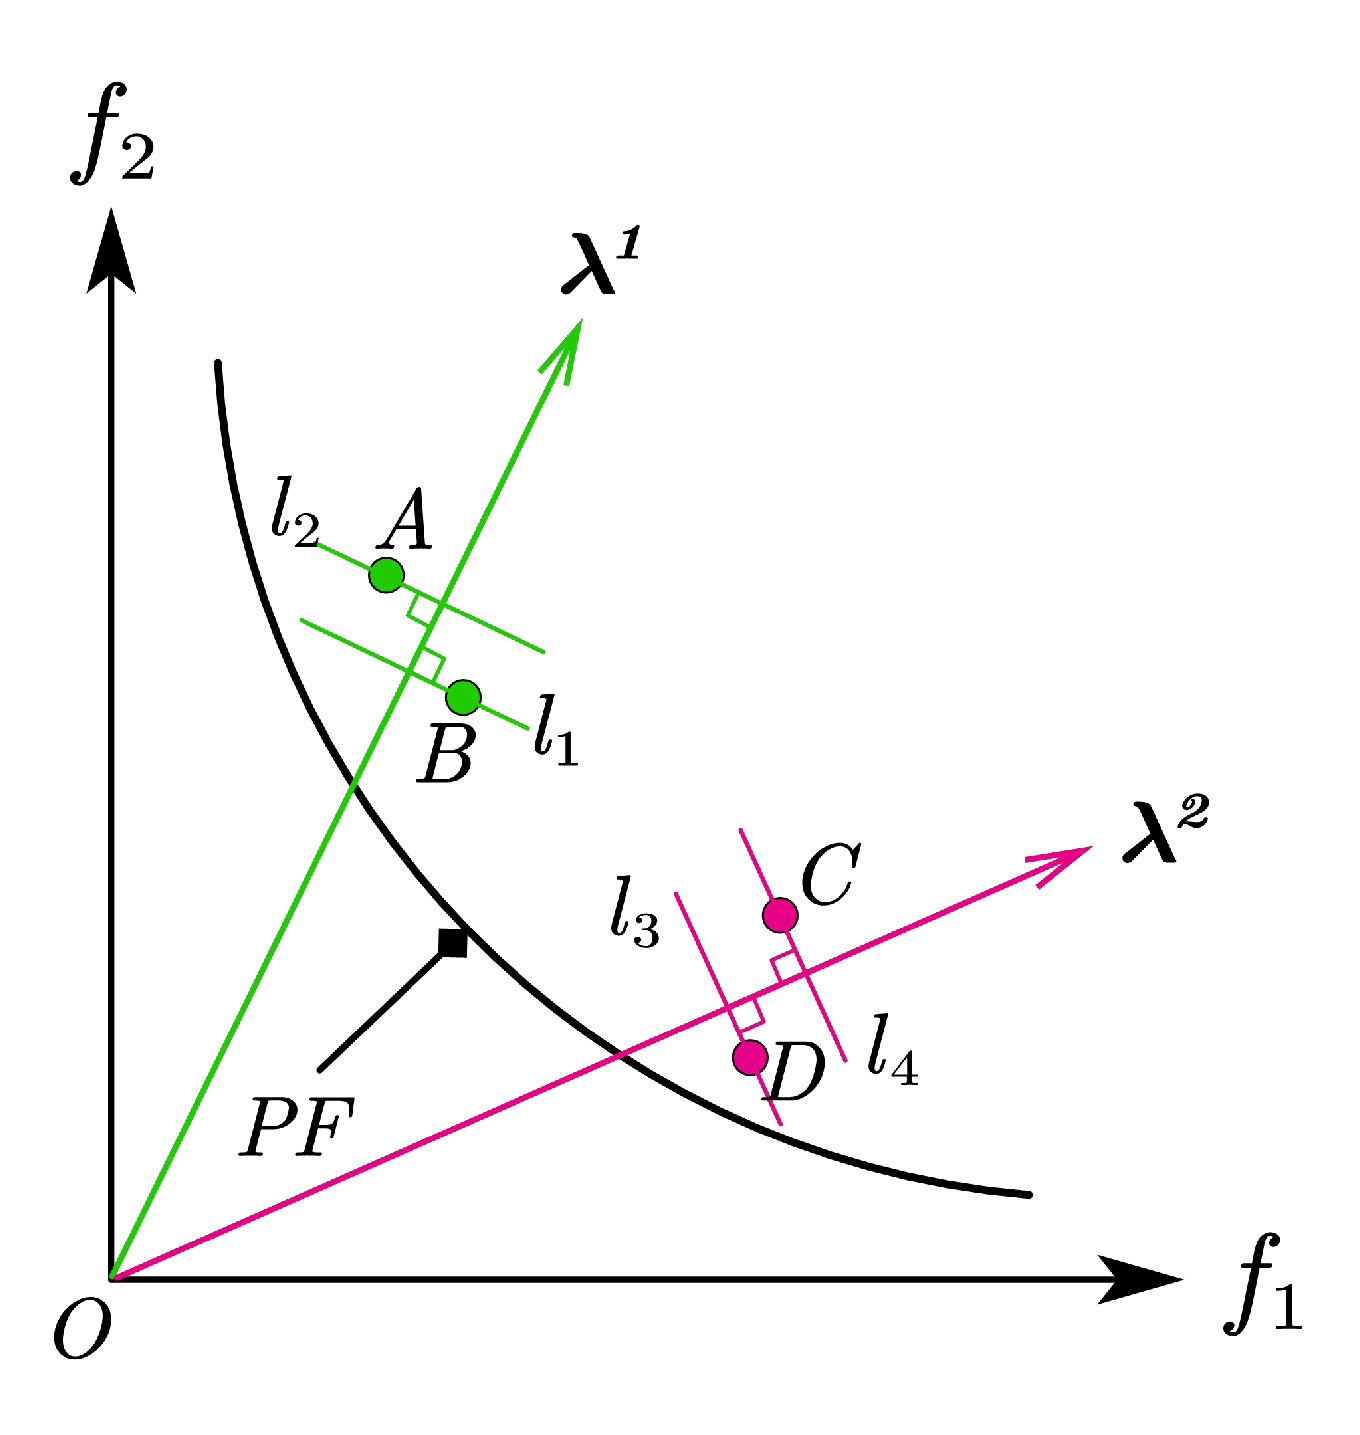
\includegraphics[width=.45\linewidth]{WS等高线.pdf}
    \caption[加权和法(WS)等高线示意图]{加权和法(WS)等高线示意图 \\ $\boldsymbol{\lambda^1}$和$\boldsymbol{\lambda^2}$分别为两个子问题的权重向量,$l_1, l_2, l_3, l_4$分别为对应子问题的等高线}
    \label{fig:WS等高线示意图}
\end{figure}
\par
\autoref{fig:WS等高线示意图}~展示的是一个二目标优化问题使用加权和法的等高线示意图。容易看出,加权和法的等高线是一簇与权重向量$\boldsymbol{\lambda}$垂直的平行直线。个体在权重向量上的投影长度即为该个体在所属$\boldsymbol{\lambda}$上的子问题的聚合值。在\autoref{fig:WS等高线示意图}~中,个体A和B是互不支配的,但是,在$\boldsymbol{\lambda^1}$所属子问题上用加权和法后,个体B要优于个体A,因为个体B在$\boldsymbol{\lambda^1}$上的投影长度要比个体A短。同理,个体D优于个体C。

\subsubsection{切比雪夫法(Tchebycheff,TCH):}

TCH是一种非线性多目标聚合方法\cite{jaszkiewicz2002performance},它的目标函数聚合形式可定义为:
\begin{align}
    \label{eq:TCH}
    minimize \quad & g^{tch}(\mathbf{x} \ | \ \boldsymbol{\lambda},\mathbf{z}^*) = \max_{1 \leq i \leq m} \lambda_i | f_i(\mathbf{x}) - z^*_i |, \\
    subject \ \ to \quad & \mathbf{x} \in \Omega. \notag
\end{align}
其中$\mathbf{x}$是决策向量,$\boldsymbol{\lambda}$为权重向量,$\mathbf{z}^*$为理想点(\autoref{def:理想点})。
\par
\begin{figure}[htb]
    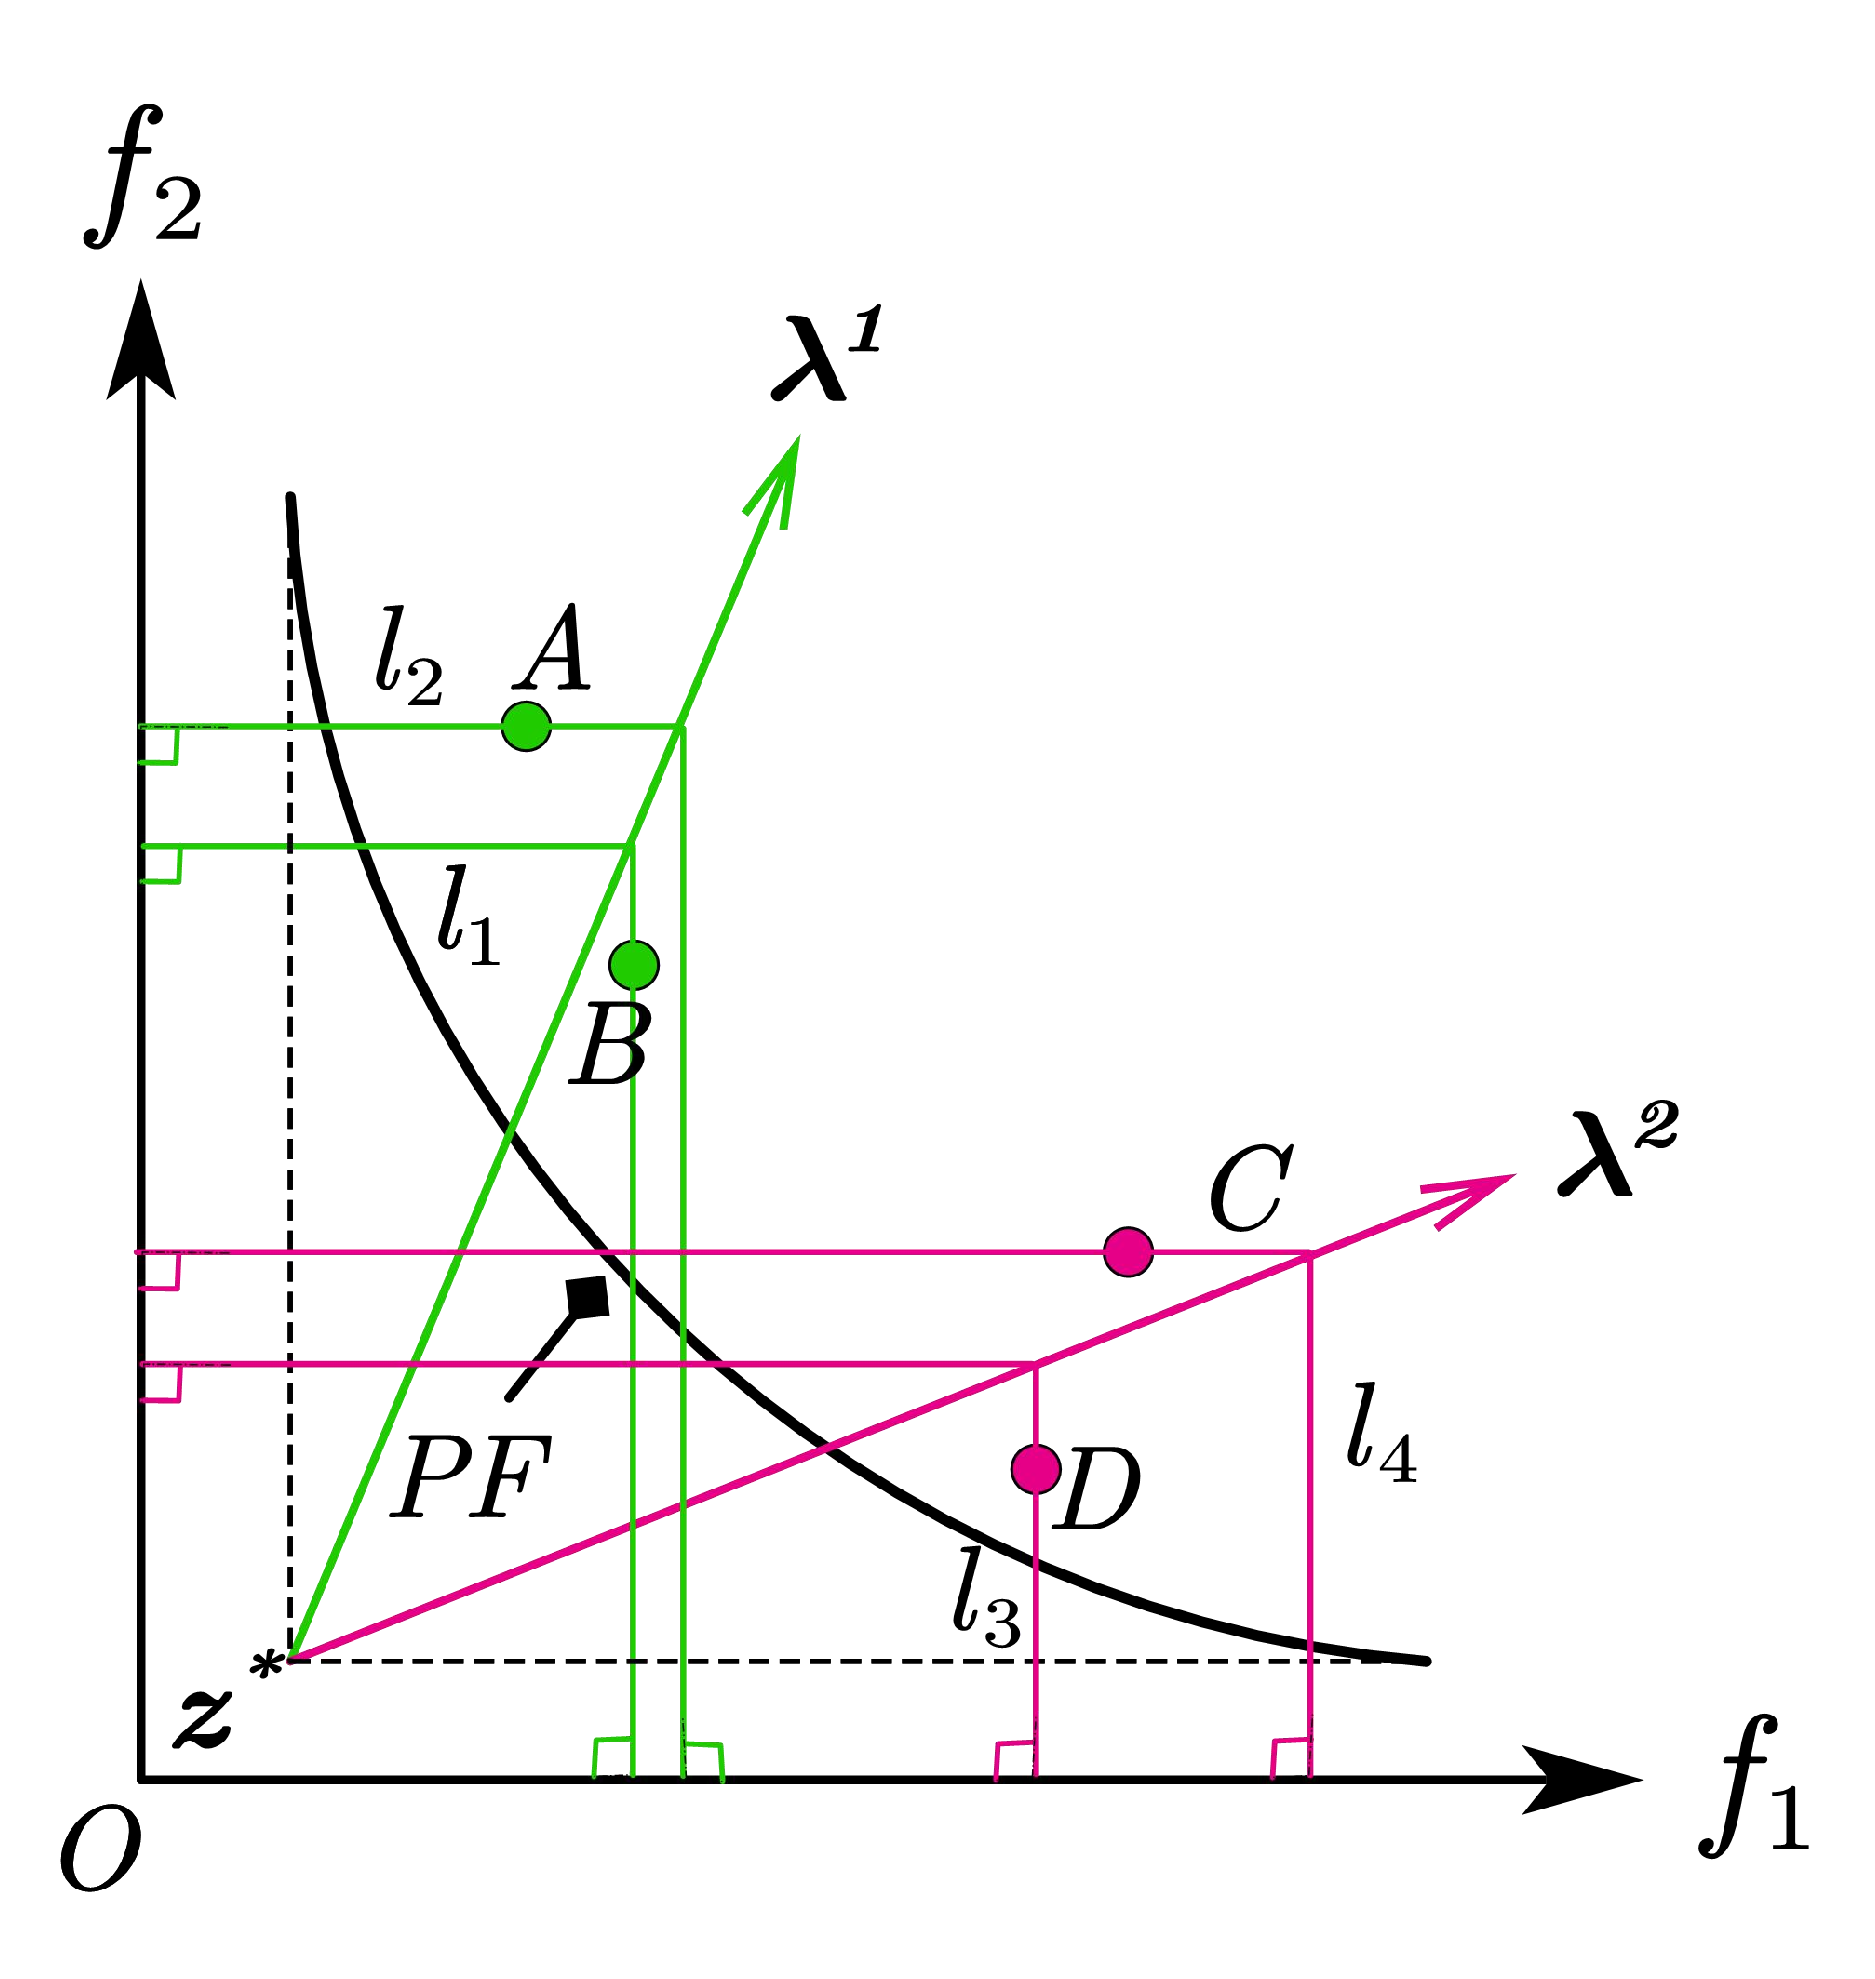
\includegraphics[width=.5\linewidth]{TCH等高线.pdf}
    \caption[切比雪夫法(TCH)等高线示意图]{切比雪夫法(TCH)等高线示意图 \\ $\boldsymbol{\lambda^1}$和$\boldsymbol{\lambda^2}$分别为两个子问题的权重向量,$l_1, l_2, l_3, l_4$分别为对应子问题的等高线}
    \label{fig:TCH等高线示意图}
\end{figure}
\par
\autoref{fig:TCH等高线示意图}~展示的是一个二目标优化问题使用切比雪夫法的等高线示意图。从    \autoref{fig:TCH等高线示意图}~中可以看出,在连续PF时,用TCH分解方法得到的子问题的最优解是权重向量与PF面的交点。在非连续PF时,由于权重向量可能和PF面没有交点,所属不同权重向量的子问题可能具有相同的最优解。相比于加权和法,TCH分解方法的等高线沿着权重向量呈直角锯齿形,因此,用TCH方法得到的子问题具有更小的收敛区域(搜索空间),这在处理高维问题时,TCH分解方法能够很好的限制收敛区域,因此能够很好的保证种群的收敛性。

\subsubsection{基于惩罚的边界交叉法(Penalty-based Boundary Intersection,PBI):}

PBI是由Zhang等人于2007年提出的一种分解方法\cite{zhang2007moea},它的目标函数聚合形式为:
\begin{align}
    \label{eq:PBI}
    minimize \quad & g^{pbi}(\mathbf{x} \ | \ \boldsymbol{\lambda},\mathbf{z}^*) = d_1 + \theta d_2, \\
    & d_1 = \frac{\| (\mathbf{z}^* - F(\mathbf{x}))^T \boldsymbol{\lambda} \Vert }{ \|  \boldsymbol{\lambda} \Vert }, \notag\\
    & d_2 = \| F(\mathbf{x}) - (\mathbf{z}^* - d_1 \boldsymbol{\lambda}) \Vert, \notag \\
    subject \ \ to \quad & \mathbf{x} \in \Omega. \notag
\end{align}
其中$\mathbf{x}$是决策向量,$\boldsymbol{\lambda}$为权重向量,$\mathbf{z}^*$为理想点(\autoref{def:理想点}),$d_1$表示目标向量$F(\mathbf{x})$到权重向量$\boldsymbol{\lambda}$的投影长度,$d_2$表示目标向量$F(\mathbf{x})$到权重向量$\boldsymbol{\lambda}$的垂直距离,$\theta$为惩罚因子,用于调节$d_1$和$d_2$之间的平衡,控制种群的分布性和收敛性。
\par
\begin{figure}[htb]
    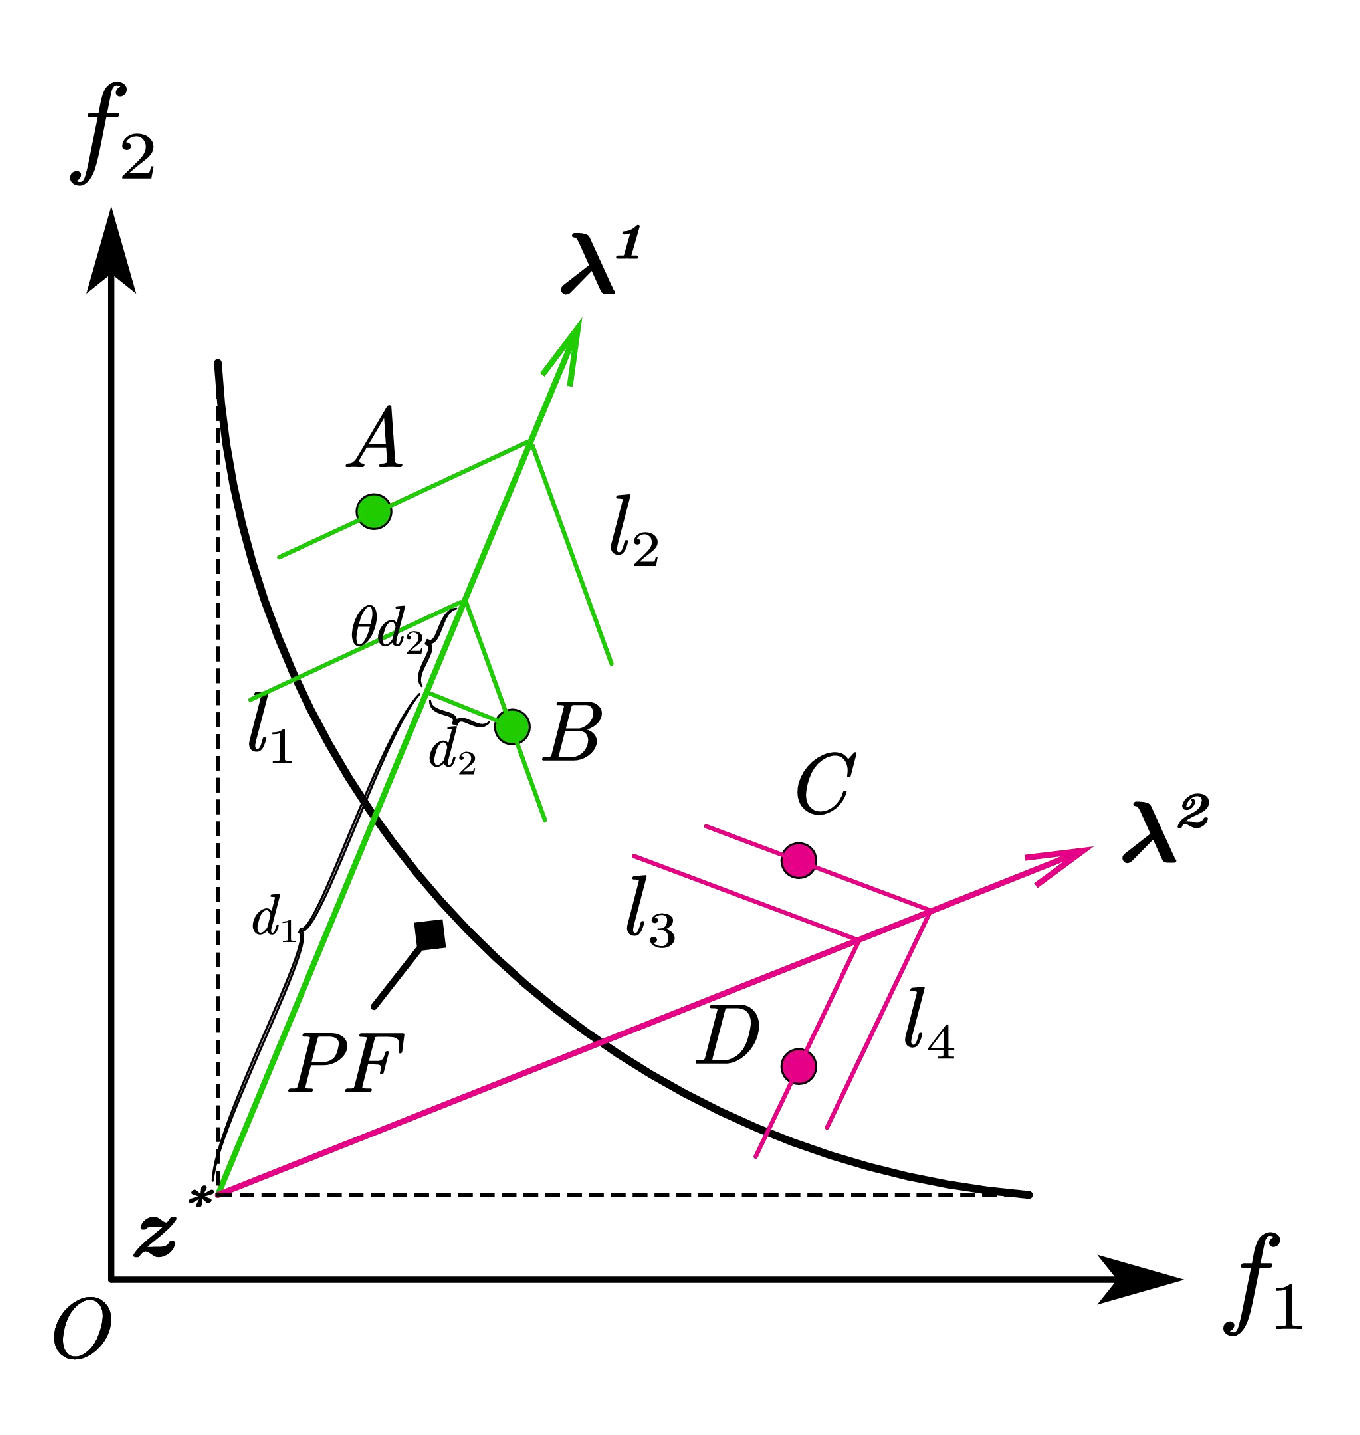
\includegraphics[width=.5\linewidth]{PBI等高线.pdf}
    \caption[基于惩罚的边界交叉法(PBI)等高线示意图]{基于惩罚的边界交叉法(PBI)等高线示意图 \\ $\boldsymbol{\lambda^1}$和$\boldsymbol{\lambda^2}$分别为两个子问题的权重向量,$l_1, l_2, l_3, l_4$分别为对应子问题的等高线}
    \label{fig:PBI等高线示意图}
\end{figure}
\par
\autoref{fig:PBI等高线示意图}~展示的是一个二目标优化问题使用基于惩罚的边界交叉法的等高线示意图。在图中,$d_1$是个体B到权重向量$\boldsymbol{\lambda^1}$的投影长度,$d_2$是个体B到权重向量$\boldsymbol{\lambda^1}$的垂直距离,$d_1+\theta d_2$即为PBI聚合值。显然,对于$\boldsymbol{\lambda^1}$所属子问题,个体B的PBI聚合值要优于个体A,即个体B优于个体A。同理,个体D优于个体C。通过\autoref{eq:PBI}~和\autoref{fig:PBI等高线示意图}~可以知道,PBI能够通过调节$\theta$参数来控制$d_1$和$d_2$之间的平衡,从而控制种群的分布性和收敛性。由于能够控制分布性和收敛性之间的平衡这一特点,PBI分解方法在处理高维目标(超多目标)问题时具有很大的优势。但是,参数$theta$的设置也影响着算法的性能表现,这同时也成为PBI分解方法的缺点之一。

\begin{figure}[htb]
    \subfloat[WS等高线示意图\label{subfig:WS等高线示意图}]{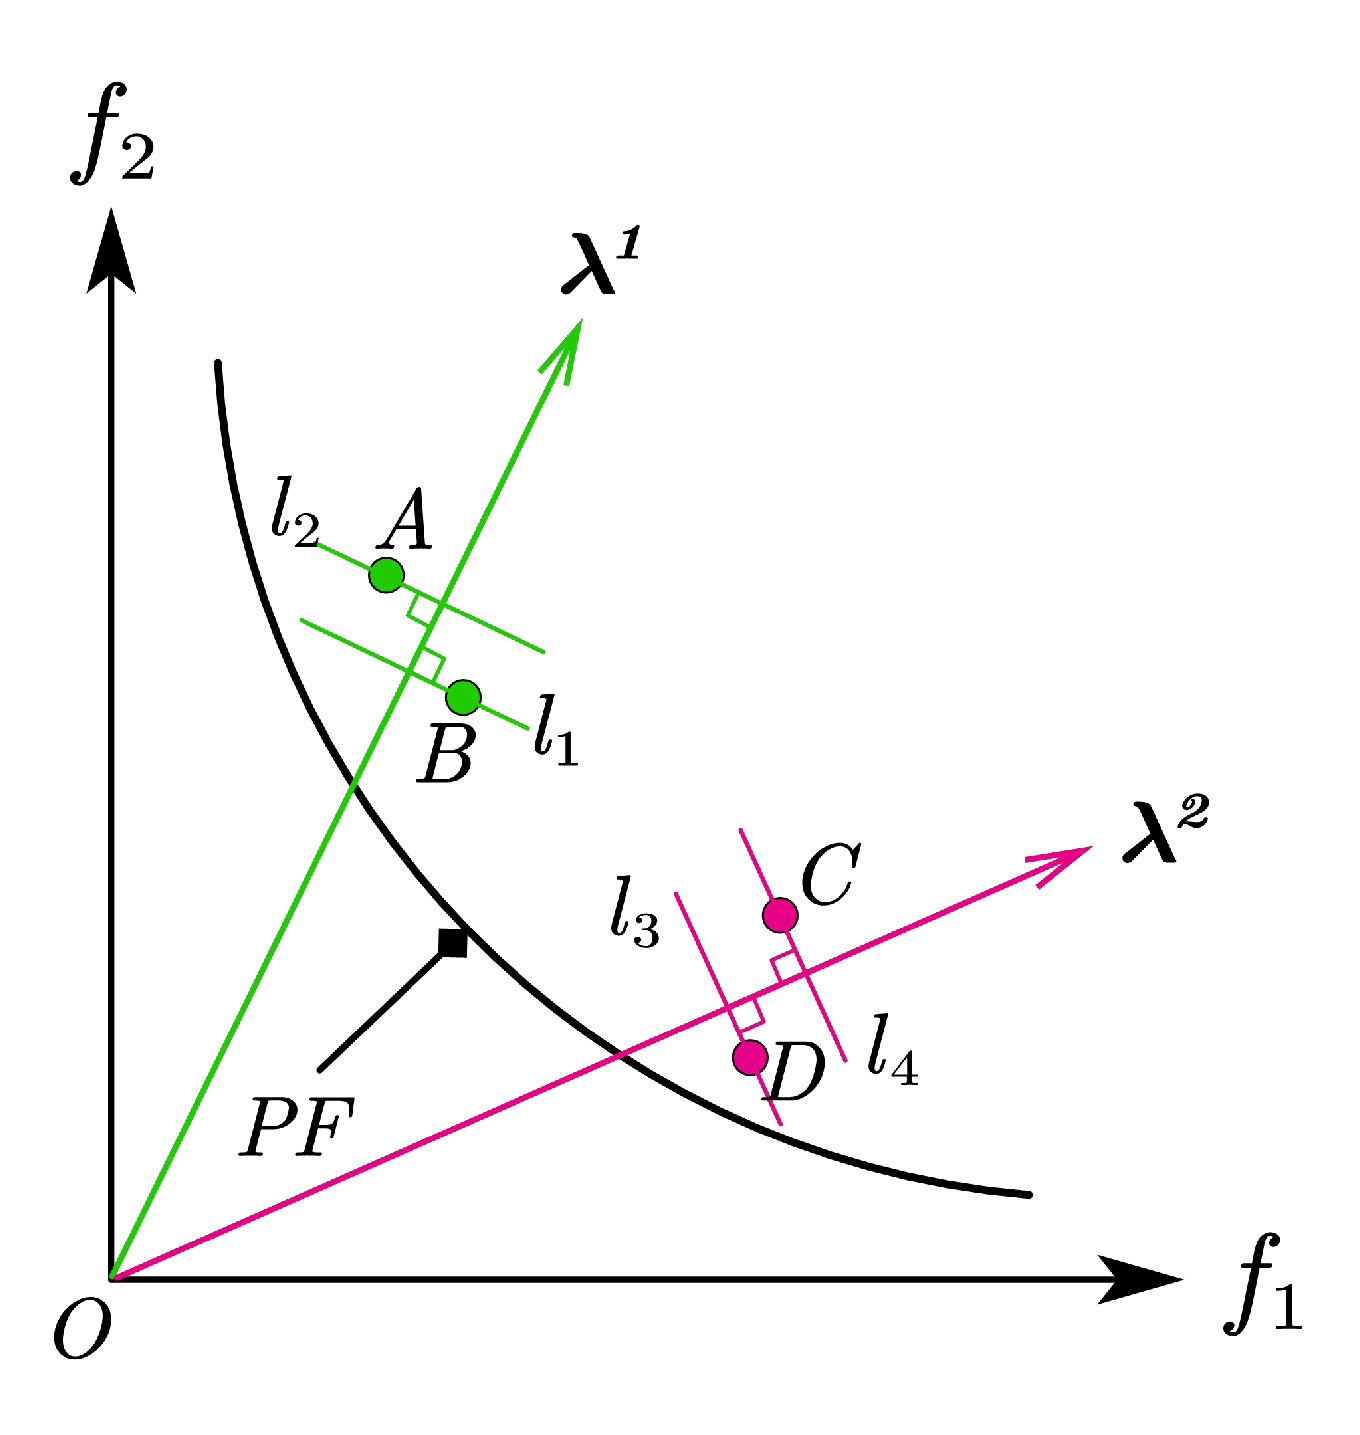
\includegraphics[width=.33\linewidth]{WS等高线.pdf}}
    \subfloat[TCH等高线示意图\label{subfig:TCH等高线示意图}]{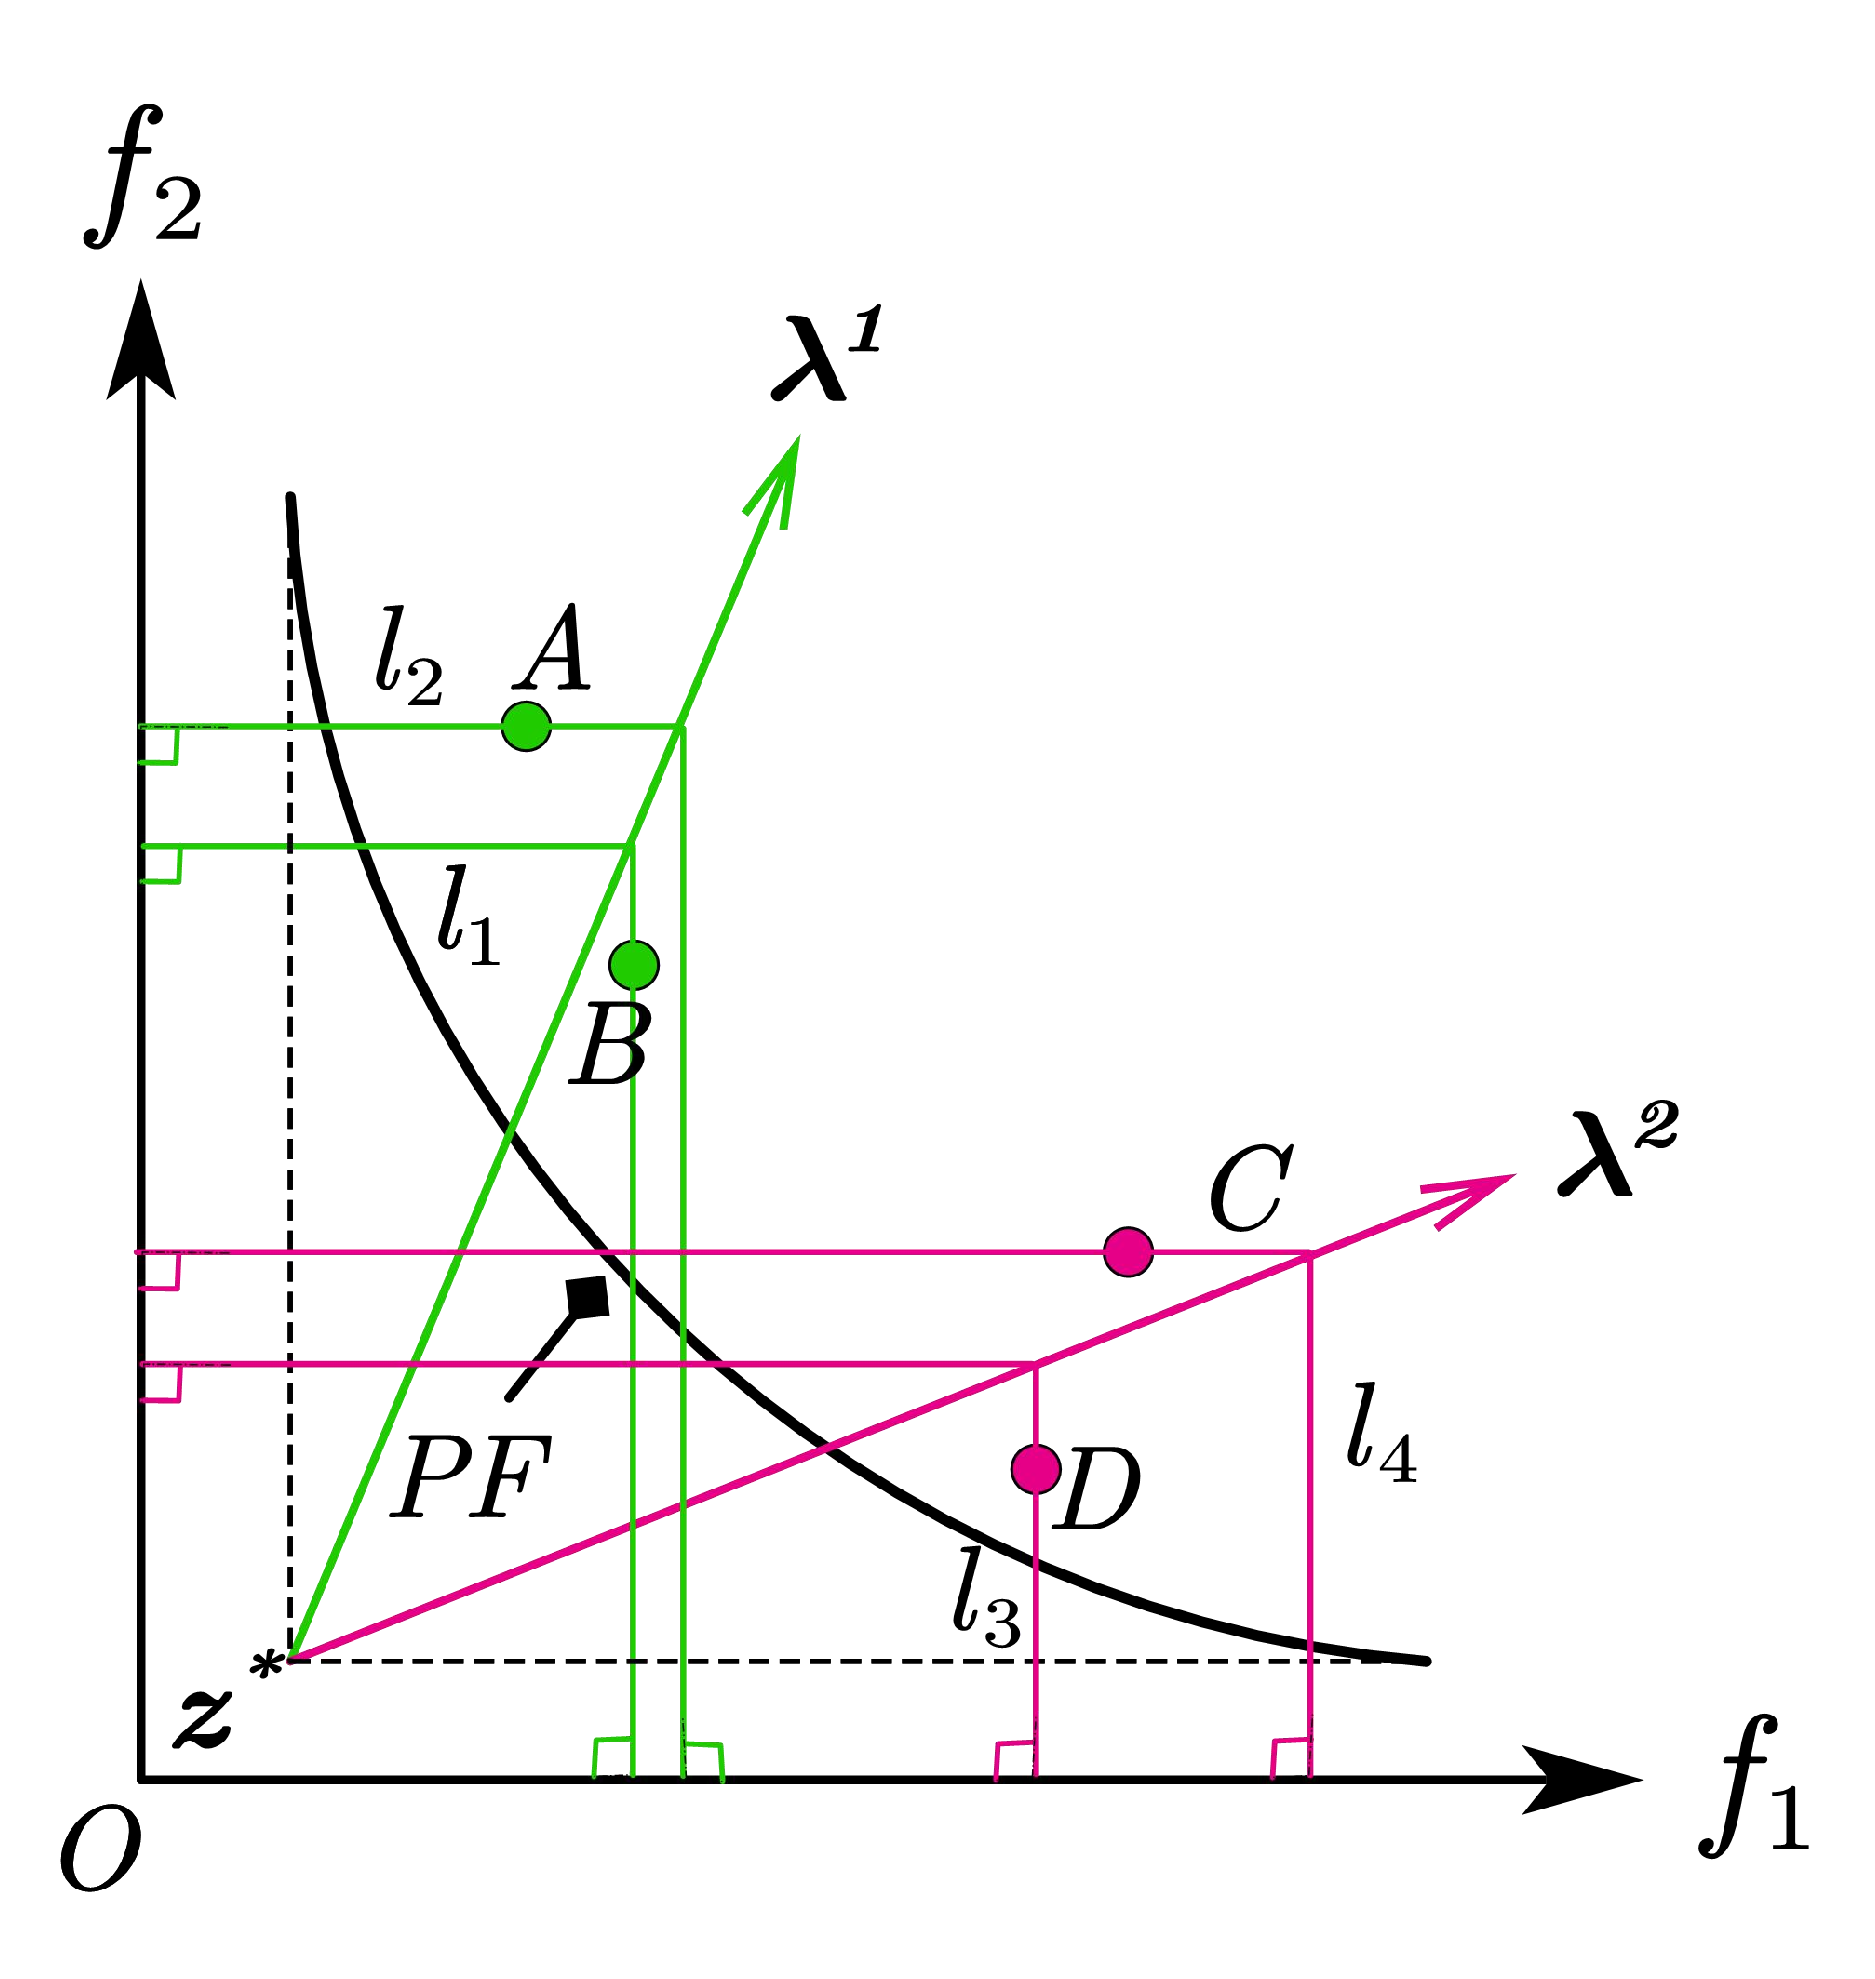
\includegraphics[width=.33\linewidth]{TCH等高线.pdf}}
    \subfloat[PBI等高线示意图\label{subfig:PBI等高线示意图}]{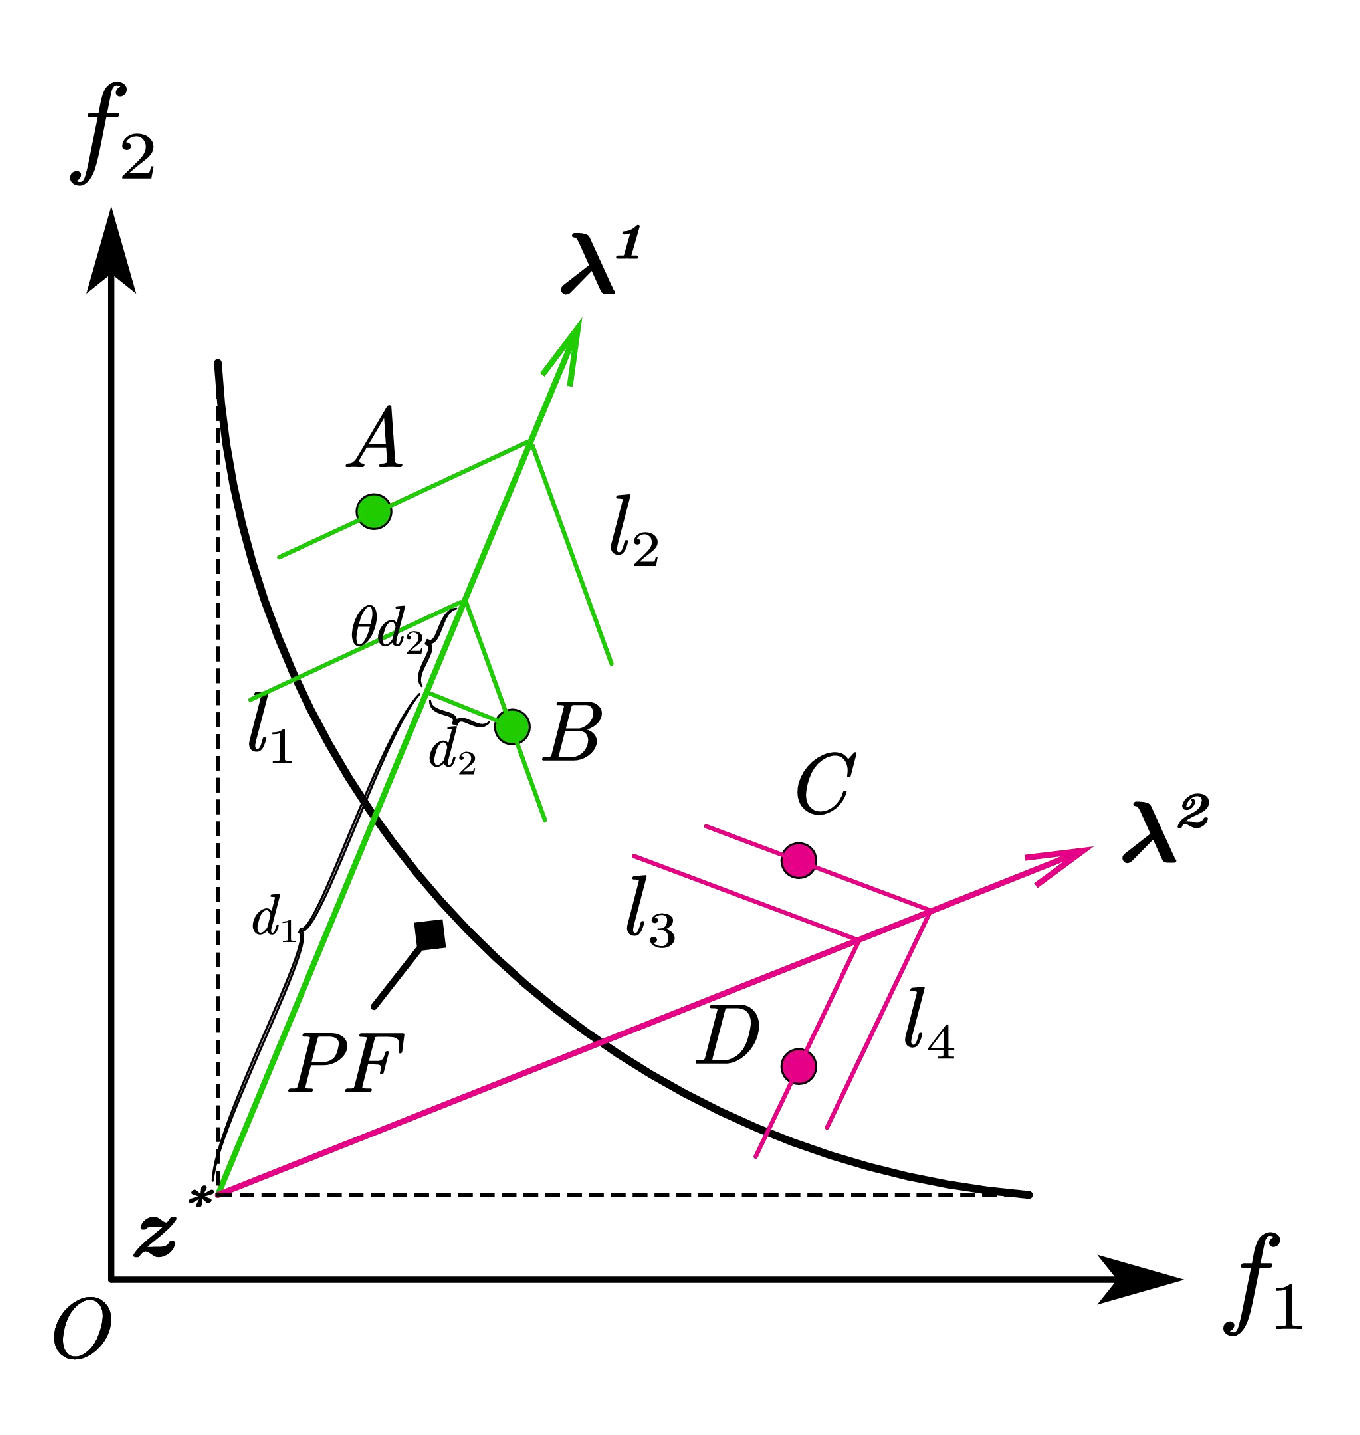
\includegraphics[width=.33\linewidth]{PBI等高线.pdf}}
    \caption{三种聚合方法等高线示意图}
    \label{fig:三种聚合方法等高线示意图}
\end{figure}